% L6a_Maxwell_Relations.pdf
\providecommand{\modre}[1]{\textcolor{NavyBlue}{#1}}
\providecommand{\cervene}[1]{\textcolor{Red}{#1}}
\providecommand{\dbar}{{\mathchar'26\mkern-12mu d}}

\section{Aplikace TD potenciálů}
\strana{L6a-1}

\subsection{Koeficienty lineární odezvy}
\begin{itemize}
  \item[--] analytická struktura termodynamiky odhaluje (nepřebernou) řadu vztahů mezi makroskopickými veličinami \\
        $\Rightarrow$ umožňuje experimentálně určit i takové, které je obtížné/nemožné měřit přímo
  \item[--] \kw{koeficienty odezvy} jsou typicky dobře měřitelné veličiny, které určují, jak se nějaká fyzikální veličina v kontrolovaném procesu mění při změně jiné veličiny
\end{itemize}
\[
  \dd X = \underbrace{\left(\pdv{X}{Y}\right)_Z}_{\text{koeficient odezvy}}\dd Y
  \quad\Rightarrow\quad X(B) - X(A) = \int_A^B\left(\pdv{X}{Y}\right)_Z\dd Y
\]

\begin{priklad}[Př:]
\begin{itemize}
  \item \kw{koeficient tepelné roztažnosti} (za konst.\ tlaku)
  \[
    \vzorec{\alpha \equiv \frac1V\left(\pdv{V}{T}\right)_p} \qquad \modre{\lessgtr 0}
  \]
  \item \kw{izotermická kompresibilita}
  \[
    \vzorec{\kappa_T \equiv -\frac1V\left(\pdv{V}{p}\right)_T} \qquad \modre{> 0 \quad \text{(ukážeme později)}}
  \]
  \modre{\phantom{xxxxxx}$\overset{\shortparallel}{\beta}$ -- časté alternativní značení}
\end{itemize}
\end{priklad}

$\Rightarrow$ celkově dostáváme pro $V = V(T,p)$
\[
  \dd V = V\alpha\,\dd T - V\kappa_T\,\dd p \tag{$*$}
\]

%----------------------------------------------------------------------
\strana{L6a-2}
\begin{itemize}
  \item co víme o $p = p(T,V)$?
\end{itemize}
\begin{align*}
  \left(\pdv{p}{T}\right)_V &= /\text{pravidlo \uv{$-1$}}/ = -\left(\pdv{V}{T}\right)_p\Big/\left(\pdv{V}{p}\right)_T = \frac{\alpha}{\kappa_T} \\
  \left(\pdv{p}{V}\right)_T &= \left[\left(\pdv{V}{p}\right)_T\right]^{-1} = -\frac{1}{V\kappa_T}
\end{align*}
\[
  \Rightarrow\quad \dd p = \frac{\alpha}{\kappa_T}\dd T - \frac{1}{V\kappa_T}\dd V \tag{$**$}
\]
$\Rightarrow$ stačí proměřit $\alpha$, $\kappa_T$ a známe i závislost tlaku na teplotě a objemu

\pozor{! ve ($*$) a ($**$) jsou $\alpha,\kappa_T$ funkce $(T,p)$ resp.\ $(T,V)$ !} \\
\quad a tuto substituci bez znalosti stavové rovnice neumíme provést $\Rightarrow$ vztahy jsou užitečné opravdu jen \uv{lokálně}

\underline{Pozorování:} (omezujeme se na uzavřené systémy, $\dd N = 0$)
\begin{itemize}[nosep]
  \item $\dd G = -S\,\dd T + V\,\dd p$
  \item $\dd F = -S\,\dd T - p\,\dd V$
\end{itemize}
\[
  \Rightarrow\quad \alpha = \frac1V\left(\frac{\partial^2G}{\partial T\,\partial p}\right)
  \qquad\&\qquad
  \kappa_T = -\frac1V\left(\frac{\partial^2G}{\partial p^2}\right)_T
\]
\[
  \Rightarrow\quad \left(\pdv{p}{T}\right)_V = -\left(\frac{\partial^2F}{\partial T\,\partial V}\right)
\]
$\Rightarrow$
\begin{enumerate}[label=\roman*)]
  \item koeficienty lin.\ odezvy lze vztáhnout k druhým derivacím vhodného TD potenciálu
  \item koeficienty odvozené z různých potenciálů nejsou nezávislé
\end{enumerate}

%----------------------------------------------------------------------
\strana{L6a-3}
$\to$ ad ii) -- \sout{toto} jistě není překvapivé -- TD pot.\ jsou svázány LT $\Rightarrow$ jsou to jen různá ekvivalentní vyjádření téhož, nenesou žádnou nezávislou informaci

$\Rightarrow$ mělo by tedy být možné vyjádřit $\forall$ druhé derivace $\forall$ TD potenciálů pomocí \uv{základní sady} odvozené z jednoho vybraného
\begin{itemize}
  \item standardně se volí $G = G(T,p)$, neboť $T,p$ lze dobře laboratorně kontrolovat:
  \[ \dd G = -S\,\dd T + V\,\dd p \]
\end{itemize}

\begin{minipage}{0.7\textwidth}
\begin{enumerate}[label=\arabic*)]
  \item $\alpha = \dfrac1V\left(\pdv{V}{T}\right)_p = \dfrac1V\left(\dfrac{\partial^2G}{\partial T\,\partial p}\right)$
        \ \modre{$= \dfrac1V\left(\dfrac{\partial^2G}{\partial p\,\partial T}\right) = -\dfrac1V\left(\pdv{S}{p}\right)_T$}
  \item $\kappa_T = -\dfrac1V\left(\pdv{V}{p}\right)_T = -\dfrac1V\left(\dfrac{\partial^2G}{\partial p^2}\right)_T$
  \item $C_p = T\left(\pdv{S}{T}\right)_p = -T\left(\dfrac{\partial^2G}{\partial T^2}\right)_p$
\end{enumerate}
\end{minipage}
\begin{minipage}{0.28\textwidth}
\centering
\fcolorbox{Red}{white}{\cervene{$\displaystyle C_X = T\left(\pdv{S}{T}\right)_X$}}

\cervene{$\Uparrow$}
\end{minipage}

\begin{minipage}{0.45\textwidth}
\modre{$\displaystyle C_V = \frac{\dbar Q}{\dd T}\Big)_V = \frac{\dd U + p\,\dd V}{\dd T}\Big)_V$ \\[2pt]
$\displaystyle \phantom{C_V} = \frac{\dd U}{\dd T}\Big)_V = T\left(\pdv{S}{T}\right)_V$}
\end{minipage}
\begin{minipage}{0.53\textwidth}
\modre{$\displaystyle C_p = \frac{\dbar Q}{\dd T}\Big|_p = \frac{\dd U + p\,\dd V}{\dd T}\Big)_p = \frac{\dd(U + pV)}{\dd T}\Big)_p = \frac{\dd H}{\dd T}\Big)_p$ \\[2pt]
$\displaystyle \phantom{C_p} = T\left(\pdv{S}{T}\right)_p$ \quad ($\Leftarrow \dd H = T\,\dd S + V\,\dd p$)}
\end{minipage}

\underline{Pozorování:} \quad $\bullet\ \left(\pdv{S}{p}\right)_T$ není další nezávislý koeficient:

$\dd G$ je úplný diferenciál $\Rightarrow$ smíšené druhé derivace jsou záměnné $\Rightarrow$
\[
  \left(\frac{\partial^2G}{\partial p\,\partial T}\right) = \left(\frac{\partial^2G}{\partial T\,\partial p}\right)
  \ \Leftrightarrow\
  \underbrace{-\left(\pdv{S}{p}\right)_T = \left(\pdv{V}{T}\right)_p}_{\text{\modre{Maxwellova relace}}}
  \ \Rightarrow\ \vzorec{\left(\pdv{S}{p}\right)_T = -V\alpha}
\]

%----------------------------------------------------------------------
\strana{L6a-4}
\subsection{Maxwellovy relace}
\begin{definice}[Maxwellovy relace]
-- rovnosti různých parciálních derivací stavových funkcí, které plynou z \kw{úplnosti diferenciálů TD potenciálů}
\end{definice}

\begin{priklad}[Př:]
\begin{enumerate}[label=\roman*)]
  \item $\dd U = T\,\dd S - p\,\dd V + \mu\,\dd N$ \\
        -- generuje 3 páry smíšených druhých derivací
  \[
    \left(\frac{\partial^2U}{\partial S\,\partial V}\right)_N = \left(\frac{\partial^2U}{\partial V\,\partial S}\right)_N
    \ \Leftrightarrow\
    \begin{aligned}[t]
      -\left(\pdv{p}{S}\right)_{V,N} &= \left(\pdv{T}{V}\right)_{S,N} \\
      \left(\pdv{\mu}{S}\right)_{V,N} &= \left(\pdv{T}{N}\right)_{S,V} \\
      \left(\pdv{\mu}{V}\right)_{S,N} &= -\left(\pdv{p}{N}\right)_{S,V}
    \end{aligned}
  \]
  \item $\dd F = -S\,\dd T - p\,\dd V + \mu\,\dd N$
  \[
    \left(\pdv{S}{V}\right)_{T,N} = \left(\pdv{p}{T}\right)_{V,N}
    \qquad
    -\left(\pdv{p}{N}\right)_{T,V} = \left(\pdv{\mu}{V}\right)_{T,N}
    \qquad
    -\left(\pdv{S}{N}\right)_{T,V} = \left(\pdv{\mu}{T}\right)_{V,N}
  \]
\end{enumerate}
\end{priklad}

\begin{itemize}
  \item mohli bychom pokračovat, ovšem vzor je jasný:
\end{itemize}
\begin{veta}[Obecný vzor]
\begin{enumerate}[label=\arabic*)]
  \item $\dd A = y_1\,\dd X_1 + y_2\,\dd X_2 + \sum_i y_i\,\dd X_i + \sum_j X_j\,\dd y_j$
  \[
    \Rightarrow\quad \vzorec{\left(\pdv{y_1}{X_2}\right)_{X_1,X_i,y_j} = \left(\pdv{y_2}{X_1}\right)_{X_2,X_i,y_j}}
  \]
  \item LT: \quad $\dd A[y_1] = -X_1\,\dd y_1 + y_2\,\dd X_2 + \dots$
  \[
    \Rightarrow\quad \vzorec{-\left(\pdv{X_1}{X_2}\right)_{y_1,X_i,y_j} = \left(\pdv{y_2}{y_1}\right)_{X_2,X_i,y_j}}
  \]
\end{enumerate}
\end{veta}

%----------------------------------------------------------------------
\strana{L6a-5}
$\Rightarrow$
\begin{enumerate}[label=\arabic*)]
  \item pro daný typ systému stačí znát diferenciál jediného TD potenciálu \\
        \underline{Př:} mg.\ systém $\Rightarrow$ $\dd U = \dots + H\,\dd M + \dots$
  \item na úrovni diferenciálů odpovídá LT prohození významu (závislá/nezávislá) v daném páru sdružených proměnných a změně znaménka u příslušného příspěvku
  \item správný potenciál identifikuji podle nez.\ proměnných:
  \[
    \left(\pdv{x}{y}\right)_{z_1,z_2} \quad\Rightarrow\quad
    \text{\parbox[t]{7cm}{hledám pot., jehož přirozenými nezávislými proměnnými jsou $y, z_1, z_2$}}
  \]
  \pozor{!} může pomoci také $A = A(x,z_1,z_2)$ \ $\Leftarrow$ derivace inv.\ funkce
  \item $\forall$ Max.\ relace přečtu přímo z příslušného diferenciálu
\end{enumerate}

\underline{Pozn!} $\bullet$ existují mnemotechniky typu \uv{magický čtverec} = \uv{Velmi Těžko zapamatovatelné Schéma} \\
\quad \modre{NEDOPORUČUJI POUŽÍVAT, postup 1--4 univerzálnější}

\subsection{Redukce derivací}
\begin{itemize}[nosep]
  \item[--] vyjádření libovolné parciální derivace pomocí zvolené sady nezávislých (+ nederivovaných stav.\ vel.)
  \item[--] spec.\ uzavřené systémy $\dbar W = -p\,\dd V$, $\dd N = 0$ \\
            (2 stupně volnosti) \quad $\Rightarrow$ \quad \fbox{$\alpha,\ \kappa_T,\ C_p$}
\end{itemize}
\hspace*{3cm}(postup viz DOPLŇKY na www)

%----------------------------------------------------------------------
\strana{L6a-6}
\begin{itemize}
  \item kromě MR máme k dispozici:
  \begin{enumerate}[label=\arabic*)]
    \item derivaci implicitní funkce (pravidlo $-1$)
    \item derivaci složené fce (řetízkové pravidlo)
    \item derivaci inverzní funkce
    \item známé diferenciály TD potenciálů
  \end{enumerate}
\end{itemize}

\begin{priklad}[Příklad \cervene{(nedělat)}]
$\bullet$ změna entropie při změně tlaku za konstantního Gibbsova potenciálu \\
\modre{(a konst.\ $N$ -- dále se rozumí implicitně)}
\[
  \left(\pdv{S}{p}\right)_{G,N} = \Big/\ \text{\modre{1) TD potenciál do čitatele}}\ \Big/
  = -\frac{\left(\pdv{G}{p}\right)_S}{\left(\pdv{G}{S}\right)_p}
\]
\[
  = \Big/\ \overset{\text{\modre{2) rozepíšu diferenciál TD potenciálu}}}{\dd U = T\,\dd S - p\,\dd V \Rightarrow \dd G = -S\,\dd T + V\,\dd p}\ \Big/ =
\]
\[
  = -\frac{-S\left(\pdv{T}{p}\right)_S + V\overbrace{\left(\pdv{p}{p}\right)_S}^{\cervene{=1}}}
          {-S\left(\pdv{T}{S}\right)_p + V\underbrace{\left(\pdv{p}{S}\right)_p}_{\cervene{=0}}}
  = \frac{V - S\left(\pdv{T}{p}\right)_S}{S\left(\pdv{T}{S}\right)_p}
\]
\hfill \cervene{$=0$ \dots\ derivace 1 nezávislé proměnné podle druhé}

a) jmenovatel: \quad
\begin{minipage}[t]{0.75\textwidth}
\modre{3) derivace s entropií převedeme do čitatele \\
3a) eliminujeme pomocí MR \\
3b) pomocí vztahu pro derivaci slož.\ fce upravíme na derivaci podle teploty $\Rightarrow T\left(\pdv{S}{T}\right)_X = C_X$}
\end{minipage}
\[
  \left(\pdv{T}{S}\right)_p \underset{\substack{\uparrow\\ \cervene{\text{inv.\ fce}}}}{=} \frac{1}{\left(\pdv{S}{T}\right)_p} = \frac{T}{C_p}
\]
\end{priklad}

%----------------------------------------------------------------------
\strana{L6a-7}
\begin{priklad}[Příklad -- pokračování]
b) čitatel
\[
  \left(\pdv{T}{p}\right)_S \overset{\text{\modre{3)}}}{=} -\frac{\left(\pdv{S}{p}\right)_T}{\left(\pdv{S}{T}\right)_p}
  = -\frac{T\left(\pdv{S}{p}\right)_T}{C_p}
  = \Bigg/\ \modre{\begin{aligned}\dd G &= -S\,\dd T + V\,\dd p \\ -\left(\pdv{S}{p}\right)_T &= \left(\pdv{V}{T}\right)_p\end{aligned}}
\]
\[
  = \frac{T\left(\pdv{V}{T}\right)_p}{C_p} = \frac{TV\alpha}{C_p}
\]
c) celkem:
\[
  \left(\pdv{S}{p}\right)_{G,\modre{N}} = \frac{V - S\left(\pdv{T}{p}\right)_S}{S\left(\pdv{T}{S}\right)_p}
  = \frac{V - STV\alpha/C_p}{ST/C_p} = \vzorec{V\,\frac{C_p - ST\alpha}{ST}}
\]
$\Rightarrow$ derivaci jsme vyjádřili pomocí $C_p, \alpha, \kappa_T$ a samotných stavových veličin
\end{priklad}

\underline{Pozn:} $\bullet$ vždy je užitečné hlídat extenzivitu \\
\quad $\to \left(\pdv{S}{p}\right)$ je extenzivní (extenzivní podle intenzivní), výsledek je také extenzivní ($\propto V$)

\begin{priklad}[Př: 1) Meyerův vztah \ {\normalfont (detailně viz www/DOPLŇKY)}]
-- co s derivací $\left(\pdv{S}{T}\right)_X$ pro $X\neq p$; spec.\ $\left(\pdv{S}{T}\right)_V$
\begin{align*}
  C_V = T\left(\pdv{S}{T}\right)_V &= \big/\ S = S(T,V) = S\big(T,p(T,V)\big)\ \big/ \\
  &= T\left(\pdv{S}{T}\right)_p + T\left(\pdv{S}{p}\right)_T\left(\pdv{p}{T}\right)_V
   = \Bigg/\ \begin{aligned}\dd G &= -S\,\dd T + V\,\dd p \\ -\left(\pdv{S}{p}\right)_T &= \left(\pdv{V}{T}\right)_p\end{aligned}\ \Bigg/ \\
  &= C_p + T\left(\pdv{V}{T}\right)_p^2\Big/\left(\pdv{V}{p}\right)_T
  \quad\Rightarrow\quad \vzorec{C_V = C_p - \frac{TV\alpha^2}{\kappa_T} < C_p}
\end{align*}
\end{priklad}

%----------------------------------------------------------------------
\strana{L6a-8}
-- poslední nerovnost plyne z faktu, že $\kappa_T > 0$

\modre{\underline{Plyne z podmínky stability}
\begin{itemize}
  \item $U(S,V,\dots)$ nabývá v rovnováze minima \\
        $\Rightarrow$ je konvexní fcí ext.\ proměnných \\
        $\Rightarrow$ $F(T,V,\dots)$ je konvexní fcí ext.\ proměnných \\
        $\Leftrightarrow$ $\dd^2F = \dd^2F(\dd V,\dots)$ je pozitivně-definitní kvadr.\ forma v diferenciálech ext.\ proměnných \\
        spec.\ \quad $\left(\dfrac{\partial^2F}{\partial V^2}\right)_{T,N} = -\left(\pdv{p}{V}\right)_T = \dfrac{1}{V\kappa_T} > 0 \ \Rightarrow\ \kappa_T > 0$
  \item stejně tak $\dd^2S$ je negativně-definitní forma
  \[
    \Rightarrow\ \left(\frac{\partial^2S}{\partial U^2}\right)_V = \left(\frac{\partial(1/T)}{\partial U}\right)_V
    = -\frac{1}{T^2}\left(\pdv{T}{U}\right)_V = -\frac{1}{T^2C_V} < 0 \ \Rightarrow\ C_V > 0
  \]
\end{itemize}
$\Rightarrow$ celkem máme \quad $C_V > 0$, \quad $C_p = C_V + TV\dfrac{\alpha^2}{\kappa_T} > C_V$ \\
\quad (pokud systém přijímá teplo za konst.\ tlaku, musí zároveň konat práci, jinak by tlak stoupal $\Rightarrow C_p > C_V$)}

\begin{priklad}[2) Sklon adiabaty a izotermy v $p$--$V$ diagramu \ {\normalfont (cf.\ Carnotův cyklus)}]
\[
  \frac{\left(\pdv{V}{p}\right)_S}{\left(\pdv{V}{p}\right)_T}
  = \Big/\ \kappa_S = -\frac1V\left(\pdv{V}{p}\right)_S\ \Big/ = \frac{\kappa_S}{\kappa_T}
  = \frac{\left(\pdv{S}{p}\right)_V}{\left(\pdv{S}{V}\right)_p}\,
    \frac{\left(\pdv{T}{V}\right)_p}{\left(\pdv{T}{p}\right)_V}
\]
\[
  \underset{\substack{\nearrow\\ \text{\modre{inverzní fce}}}}{=}
  \frac{\left(\pdv{S}{p}\right)_V\left(\pdv{p}{T}\right)_V}{\left(\pdv{S}{V}\right)_p\left(\pdv{V}{T}\right)_p}
  \overset{\text{\modre{slož.\ fce}}}{=}
  \frac{\left(\pdv{S}{T}\right)_V}{\left(\pdv{S}{T}\right)_p} = \frac{C_V}{C_p}
  \quad\Rightarrow\quad \vzorec{\frac{\kappa_S}{\kappa_T} = \frac{C_V}{C_p} < 1}
\]
\end{priklad}

%----------------------------------------------------------------------
\strana{L6a-9}
\begin{minipage}{0.5\textwidth}
\[
  \Rightarrow\ \frac{\left(\pdv{V}{p}\right)_S}{\left(\pdv{V}{p}\right)_T}
  = \frac{\left(\pdv{p}{V}\right)_T}{\left(\pdv{p}{V}\right)_S} < 1 \quad\Rightarrow
\]
\end{minipage}
\begin{minipage}{0.48\textwidth}
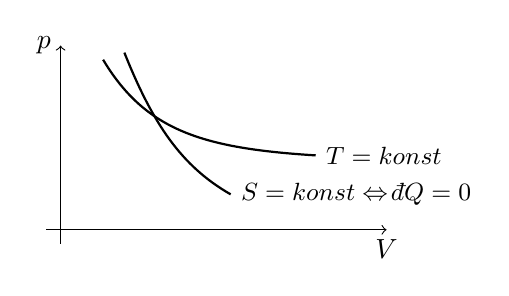
\begin{tikzpicture}[scale=0.9]
  \draw[->] (0,-0.2) -- (0,2.6) node[left] {$p$};
  \draw[->] (-0.2,0) -- (4.6,0) node[below] {$V$};
  % izoterma (pozvolnější)
  \draw[thick] (0.6,2.4) .. controls (1.2,1.4) and (2,1.15) .. (3.6,1.05) node[right] {\small $T = \text{konst}$};
  % adiabata (strmější)
  \draw[thick] (0.9,2.5) .. controls (1.3,1.5) and (1.7,0.9) .. (2.4,0.5) node[right] {\small $S = \text{konst} \Leftrightarrow \dbar Q = 0$};
\end{tikzpicture}
\end{minipage}

\quad $\to$ obrázek pro Carnotův cyklus byl správně! \\
\quad (nebylo to však zásadní; důležité bylo, aby $\dd T = 0$ a $\dbar Q = 0$ nesplývaly)

\noindent\rule{\linewidth}{0.4pt}

\subsection{Aplikace}
\begin{priklad}[1) Volná expanze do vakua]
\begin{minipage}{0.42\textwidth}
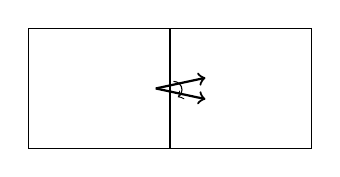
\begin{tikzpicture}[scale=0.9]
  \draw (0,0) rectangle (4,1.7);
  \draw (2,0) -- (2,1.7);
  \draw[->,thick] (1.8,0.85) -- (2.5,1.0);
  \draw[->,thick] (1.8,0.85) -- (2.5,0.7);
  \draw[->] (2.05,0.95) arc (90:-60:0.12);
\end{tikzpicture}
\end{minipage}
\begin{minipage}{0.56\textwidth}
$U = \text{konst} \ \Rightarrow\ \Delta T = \displaystyle\int_{V_0}^{V_f}\left(\pdv{T}{V}\right)_{U,N}\dd V$
\[
  \vzorec{\dd T = \left(\pdv{T}{V}\right)_{U,N}\dd V}
\]
\end{minipage}

\begin{align*}
  \left(\pdv{T}{V}\right)_U &= -\frac{\left(\pdv{U}{V}\right)_T}{\left(\pdv{U}{T}\right)_V}
  = -\frac{T\left(\pdv{S}{V}\right)_T - p}{T\left(\pdv{S}{T}\right)_V}
  = \big/\ \dd F = -S\,\dd T - p\,\dd V\ \big/ \\
  &= -\frac{T\left(\pdv{p}{T}\right)_V - p}{C_V} = -\frac{1}{C_V}\left(T\frac{\alpha}{\kappa_T} - p\right)
  = \vzorec{\mu_J} \quad \text{(Jouleův koeficient)}
\end{align*}
\begin{minipage}{0.5\textwidth}
\[
  \Rightarrow\ \Delta T = -\int_{V_1}^{V_2}\frac{1}{C_V}\left(T\frac{\alpha}{\kappa_T} - p\right)\dd V
\]
\end{minipage}
\begin{minipage}{0.48\textwidth}
\modre{$\forall$ veličiny pod integrálem nutno vyjádřit jako fce $V$ pro dané $U = \text{konst}$: \\
$T = T(V)$, $\alpha = \alpha(V)$, \dots}
\end{minipage}
\end{priklad}

\underline{Pozn:}
\begin{itemize}[nosep]
  \item pokud bychom znali $U = U(T,V)$, potom je samozřejmě lépe využít $U(T_1,V_1) = U(T_2,V_2)$
  \item pro malé změny platí \quad $\Delta T \simeq -\dfrac{1}{C_V}\left(T\dfrac{\alpha}{\kappa_T} - p\right)\bigg|_{V = V_0}\Delta V$
\end{itemize}

%----------------------------------------------------------------------
\strana{L6a-10}
\underline{Id.\ plyn:}
\begin{align*}
  U &= cNk_BT \ \Rightarrow\ C_V = cNk_B \\
  V &= \frac{Nk_BT}{p} \ \Rightarrow\ \alpha = \frac{Nk}{Vp} = \frac1T \quad\&\quad \kappa_T = \frac{Nk_BT}{p^2V} = \frac1p
\end{align*}
\[
  \Rightarrow\ \mu_J = -\frac{1}{cNk_B}\left(T\frac{p}{T} - p\right) = 0
\]
\quad $\Rightarrow$ pro id.\ plyn se teplota nemění \quad \checkmark

\begin{minipage}{0.4\textwidth}
\underline{vdW plyn:}
\end{minipage}
\begin{minipage}{0.28\textwidth}
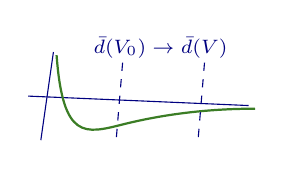
\begin{tikzpicture}[scale=0.8]
  \draw[NavyBlue] (-0.1,-0.7) -- (0.1,0.7);
  \draw[NavyBlue] (-0.3,0) -- (3.2,-0.15);
  \draw[OliveGreen,thick] (0.15,0.65) .. controls (0.25,-0.7) and (0.6,-0.6) .. (1.2,-0.45)
        .. controls (1.8,-0.3) and (2.5,-0.2) .. (3.3,-0.2);
  \draw[NavyBlue,dashed] (1.1,-0.65) -- (1.2,0.55);
  \draw[NavyBlue,dashed] (2.4,-0.65) -- (2.5,0.55);
  \node[NavyBlue,above] at (1.8,0.45) {\scriptsize $\bar d(V_0)\to\bar d(V)$};
\end{tikzpicture}
\end{minipage}
\begin{minipage}{0.3\textwidth}
\modre{\small (při expanzi interagujících částic vzroste střední hodnota pot.\ energie) $\Rightarrow$ klesne střední kin.\ energie}
\end{minipage}

\underline{cvičení:} \quad $\mu_J = -\dfrac{a}{C_V}\left(\dfrac{n}{V}\right)^2 < 0 \ \Rightarrow$ plyn se ochladí
\hfill \modre{\small $\updownarrow$ další příklad}

\begin{minipage}{0.68\textwidth}
-- efektivitu ochlazení určuje koef.\ $a$ -- míra interakcí mezi částicemi
\end{minipage}
\begin{minipage}{0.3\textwidth}
\modre{\small $S\nearrow \Leftrightarrow \bar E\nearrow$ \\ $\Rightarrow$ entropický a energ.\ princip \uv{soupeří}}
\end{minipage}

\cervene{$\downarrow$ cvičení}
\begin{priklad}[2) Jouleův--Thomsonův proces \ {\normalfont (throttling)}]
\begin{center}
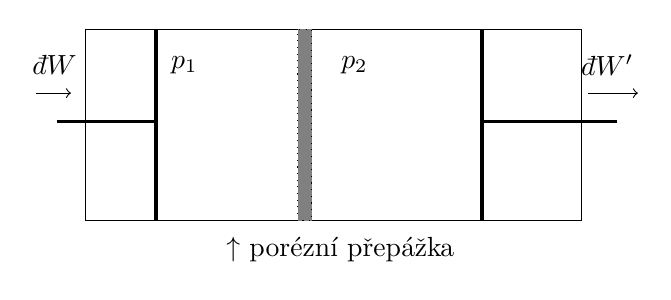
\begin{tikzpicture}[scale=0.9]
  \draw (0,0) rectangle (7,2.7);
  % levý píst
  \draw[very thick] (1,0) -- (1,2.7);
  \draw[very thick] (-0.4,1.4) -- (1,1.4);
  \node at (-0.4,2.2) {$\dbar W$};
  \draw[->] (-0.7,1.8) -- (-0.2,1.8);
  \node at (1.4,2.2) {$p_1$};
  % porézní přepážka
  \fill[gray] (3.0,0) rectangle (3.2,2.7);
  \draw[dotted] (3.0,0) rectangle (3.2,2.7);
  \node at (3.8,2.2) {$p_2$};
  % pravý píst
  \draw[very thick] (5.6,0) -- (5.6,2.7);
  \draw[very thick] (5.6,1.4) -- (7.5,1.4);
  \node at (7.4,2.2) {$\dbar W'$};
  \draw[->] (7.1,1.8) -- (7.8,1.8);
  \node[below] at (3.6,-0.1) {$\uparrow$ porézní přepážka};
\end{tikzpicture}
\end{center}

\begin{minipage}{0.7\textwidth}
\begin{itemize}
  \item \underline{počáteční stav}: \quad $p_1, V_1$ \ \& \ $V_2 = 0$ \\
        \hspace*{2.5cm}$\to$ vnitřní energie $U_1$
  \item \underline{koncový stav}: \quad $V_1 = 0$ \ \& \ $p_2, V_2$ \\
        \hspace*{2.5cm}$\to$ $U_1 + p_1V_1 - p_2V_2 = U_2$
  \item $\Rightarrow$ \quad $U_1 + p_1V_1 = U_2 + p_2V_2 \ \Leftrightarrow\ \vzorec{H_1 = H_2}$
\end{itemize}
\end{minipage}
\begin{minipage}{0.28\textwidth}
\centering
\fbox{$\Delta p = p_2 - p_1 < 0$}
\end{minipage}
\end{priklad}

%----------------------------------------------------------------------
\strana{L6a-11}
\begin{itemize}
  \item proces reálně izoentalpický není (je \underline{nerovnovážný}) \\
        stejně jako u volné expanze platí rovnost jen na začátku a na konci
  \item pro malý rozdíl tlaků \quad $\Delta T = \left(\pdv{T}{p}\right)_H\Delta p \equiv \mu_{JT}\Delta p$
  \item pro $\Delta p$ velké lze opět integrovat:
  \[ \Delta T = \int_{p_1}^{p_2}\mu_{JT}(p)\,\dd p \]
  ($T, p, H$ jsou stavové veličiny $\Rightarrow$ mohu skutečný nerovnovážný proces nahradit \modre{libovolnou!} kvazistatickou trajektorií)
\end{itemize}
\[
  \to\ \left(\pdv{T}{p}\right)_H = -\frac{\left(\pdv{H}{p}\right)_T}{\left(\pdv{H}{T}\right)_p}
  = -\frac{T\left(\pdv{S}{p}\right)_T + V}{T\left(\pdv{S}{T}\right)_p}
  = \Big/\ \left(\pdv{S}{p}\right)_T \overset{\text{Gibbs}}{=} -\left(\pdv{V}{T}\right)_p\ \Big/
\]
\[
  = \frac{TV\alpha - V}{C_p} \quad\Rightarrow\quad \vzorec{\mu_{JT} = \frac{V}{C_p}\,(T\alpha - 1)}
\]
\begin{itemize}
  \item pro id.\ plyn \ $\alpha = \frac1T$ \ $\Rightarrow$ opět $\mu_{JT} = 0$
  \item \underline{reálné plyny}:
  \begin{enumerate}[label=\alph*)]
    \item $\alpha(T) > T^{-1} \ \Rightarrow\ \mu_{JT} > 0 \ \Rightarrow$ chlazení
    \item $\alpha(T) < T^{-1} \ \Rightarrow\ \mu_{JT} < 0 \ \Rightarrow$ zahřívání
  \end{enumerate}
\end{itemize}

\begin{definice}[Teplota inverze]
\kw{TEPLOTA INVERZE} \quad $\vzorec{T_{\mathrm{inv}}\,\alpha(T_{\mathrm{inv}}) = 1}$
\begin{itemize}[nosep]
  \item[--] pro \ $T < T_{\mathrm{inv}}$ \ chlazení \\
            \phantom{pro} \ $T > T_{\mathrm{inv}}$ \ ohřívání
\end{itemize}
(viz cvičení a J--T s vdW plynem)
\end{definice}

%----------------------------------------------------------------------
\strana{L6a-12}
\begin{priklad}[3) Práce v izotermickém procesu]
$\bullet$ úlohy 6.2-2 \& 6.2-3 v [Callen], str.\ 160

\underline{6.2-3}

\begin{minipage}{0.48\textwidth}
\centering
$T = \text{konst}$ \\[2pt]
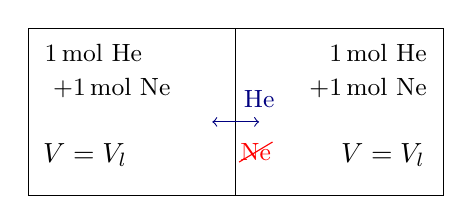
\begin{tikzpicture}[scale=0.85]
  \draw (0,0) rectangle (6.2,2.5);
  \draw (3.1,0) -- (3.1,2.5);
  \node[align=left,anchor=north west] at (0.1,2.4) {\small 1\,mol He \\ \small \ +1\,mol Ne};
  \node[align=right,anchor=north east] at (6.1,2.4) {\small 1\,mol He \\ \small +1\,mol Ne};
  \node at (0.85,0.6) {$V = V_l$};
  \node at (5.3,0.6) {$V = V_l$};
  \node[NavyBlue] at (3.45,1.45) {\small He};
  \draw[NavyBlue,<->] (2.75,1.1) -- (3.45,1.1);
  \node[Red] at (3.4,0.65) {\small \sout{Ne}};
  \draw[Red] (3.15,0.5) -- (3.65,0.8);
\end{tikzpicture}
\end{minipage}
\begin{minipage}{0.5\textwidth}
$V_l = 10\,\ell$; jakou práci musíme vykonat, abychom posunuli píst tak, že $V_L = 5\,\ell$ \& $V_R = 15\,\ell$?
\end{minipage}

\medskip
1) Víme (cvičení), že
\begin{align*}
  F_{R,L}(T,V,N_1,N_2) &= F_{R,L}(T,V,N_1) + F_{R,L}(T,V,N_2) \\
  \&\quad F(T,V,N) &= Nk_BT\left\{f_0 - \log\left[\left(\frac{T}{T_0}\right)^c\left(\frac{V}{V_0}\right)\left(\frac{N_0}{N}\right)\right]\right\}
\end{align*}
\begin{align*}
  \Rightarrow\ F_R &= N_1^Rk_BT\left\{f_0 - \log\left[\left(\tfrac{T}{T_0}\right)^c\left(\tfrac{V^R}{V_0}\right)\left(\tfrac{N_0}{N_1^R}\right)\right]\right\}
   + N_2^Rk_BT\left\{f_0 - \log\left[\left(\tfrac{T}{T_0}\right)^c\left(\tfrac{V^R}{V_0}\right)\left(\tfrac{N_0}{N_2^R}\right)\right]\right\} \\
  &= (N_1^R + N_2^R)k_BT\left\{f_0 - \log\left(\tfrac{T}{T_0}\right)^c\right\}
   - N_1^Rk_BT\log\left[\left(\tfrac{V^R}{V_0}\right)\left(\tfrac{N_0}{N_1^R}\right)\right] \\
  &\quad - N_2^Rk_BT\log\left[\left(\tfrac{V^R}{V_0}\right)\left(\tfrac{N_0}{N_2^R}\right)\right]
  \qquad\qquad N_2 \dots \text{Ne} \Rightarrow N_2^R = N_2^L = \text{fix}
\end{align*}
\begin{align*}
  \Rightarrow\ F_{\text{celk}} &= Nk_BT\left(f_0 - \log\left(\tfrac{T}{T_0}\right)^c\right)
   - N_1^Rk_BT\log\left[\left(\tfrac{V^R}{V_0}\right)\left(\tfrac{N_0}{N_1^R}\right)\right] \\
  &\quad - \tfrac12N_2k_BT\log\left[\left(\tfrac{V^R}{V_0}\right)\left(\tfrac{2N_0}{N_2}\right)\right]
   - N_1^Lk_BT\log\left[\left(\tfrac{V^L}{V_0}\right)\left(\tfrac{N_0}{N_1^L}\right)\right] \\
  &\quad - \tfrac12N_2k_BT\log\left[\left(\tfrac{V^L}{V_0}\right)\left(\tfrac{2N_0}{N_2}\right)\right]
\end{align*}

$\bullet$ \underline{rovnováha vůči výměně He}: \quad $N_1^L = N_1 - N_1^R$ \ \& \ $\dfrac{\partial F}{\partial N_1^R} = 0$!
\[
  -k_BT\log\left[\left(\tfrac{V^R}{V_0}\right)\left(\tfrac{N_0}{N_1^R}\right)\right] + k_BT
  + k_BT\log\left[\left(\tfrac{V^L}{V_0}\right)\tfrac{N_0}{N_1 - N_1^R}\right] - k_BT = 0
\]
\[
  \Rightarrow\ \log\left(\frac{V_L}{V_R}\,\frac{N_1^R}{N_1 - N_1^R}\right) = 0
  \ \Rightarrow\ \frac{N_1^R}{N_1 - N_1^R} = \frac{V_R}{V_L}
  \ \Rightarrow\ \frac{V^L}{N_1^L} = \frac{V^R}{N_1^R}
\]
\end{priklad}

%----------------------------------------------------------------------
\strana{L6a-13}
\begin{align*}
  \Rightarrow\ &N_1^Rk_BT\log\left[\frac{V^R}{N_1^R}\frac{N_0}{V_0}\right] + N_1^Lk_BT\log\left[\frac{V_L}{N_1^L}\frac{N_0}{V_0}\right] \\
  &= N_1k_BT\log\left[\frac{V^R}{N_1^R}\frac{N_0}{V_0}\right]
  \qquad\&\qquad \frac{V^R}{N_1^R} = \frac{V}{N_1}: \quad V = V^R + V^L
\end{align*}
\[
  \frac{V^R + V^L}{N_1^R + N_1^L} = \frac{V^R + V^R\frac{N_1^L}{N_1^R}}{N_1^R + N_1^L} = \frac{V^RN_1}{N_1^RN_1} = \frac{V^R}{N_1^R}
\]

\begin{tcolorbox}[colback=white,colframe=black,boxrule=0.5pt,sharp corners]
\[
  \Rightarrow\ F = Nk_BT\left(f_0 - \log\left(\frac{T}{T_0}\right)^c\right)
  - \frac12N_2k_BT\log\left[\frac{V^RV^L}{V_0^2}\,\frac{4N_0^2}{N_2^2}\right]
  - N_1k_BT\log\left(\frac{V}{V_0}\frac{N_0}{N_1}\right)
\]
\modre{Tento potenciál zahrnuje rovnováhu vůči výměně tepla i částic (He) mezi komorami}
\end{tcolorbox}

$\Rightarrow$ jediný proměnný příspěvek je \quad $-\frac12N_2k_BT\log\left(\dfrac{V^RV^L}{V_0^2}\right)$
\[
  \Rightarrow\ \underset{\substack{\shortparallel\\ \cervene{[W]_T\ !}}}{\Delta F}
  = -\frac12N_2k_BT\log\Bigg[\underbrace{\frac{5\cdot15}{10^2}}_{\uparrow\ \frac{(V^RV^L)}{(V^RV^L)_i}}\Bigg]
  = \frac12N_2k_BT\log\left(\frac43\right)
\]
$\bullet$ spec.\ \ $N_2 = 2N_A$ \quad $\Rightarrow$ \quad $\vzorec{W = RT\log\left(\tfrac43\right)}$

\underline{Cv:} zkuste spočítat práci přímo integrací

\begin{priklad}[Callen str.\ 160, 6.2-2]
V nádobě rozdělené pístem se nachází v každé komoře 1 mol vdW plynu. Oba plyny mají stejné parametry \uv{$c$} a \uv{$b$}, ale různé konstanty \uv{$a$}:
\[
  p = \frac{RT}{(v - b)} - \frac{a_i}{v^2} \qquad u = cRT - \frac{a_i}{v}
\]
Celý systém je v kontaktu s lázní o teplotě $T$. Jakou práci plyn vykoná, pokud nádoba zdvojnásobí objem a přitom vnitřní píst udržuje mechanickou rovnováhu mezi komorami?
\end{priklad}

